\chapter{Context}
People have always wanted to stay in contact with one another. Since the introduction of the internet it has never been so easy, at first we used primarily email for communication with one another over the internet, but this was a technology adapted from letters. Early social media examples can be found in early instant messengers like MSN Messenger which allowed the user to instantly communicate with one another across the world. But instant messenger platforms would be rapidly be replaced by other more robust sites such as Facebook(2004), Flickr(2004), Bebo(2005) and MySpace(2005) to name a few. These sites revolutionized how we communicate today by giving us an online presence that others can find us and communicate with us.

\section{Early Electronic Communication}
Early on when the internet was just starting off it was used to connect universities and colleges together called the ARPANET. This evolved quickly into the internet we know today. As the internet progressed from a relatively small network between 3rd level institutions, to slowly entering peoples houses where everyone could connect to this one network. Early internet used telecommunications line and shared bandwidth with phones. This stage of internet infrastructure was called dial-up. Dial-up was extremely slow with a maximum speed of 56Kbit/s, this slow speed and shared cable with a phone line made instant messaging slow and not very viable.

During this era emails were the main method of communication, it was text only and didn't require the user to be on their PC when the user sends the email. Email during this time was easy for users to understand during the early stage of home computers as it was just an electronic letter or e-mail. This allowed people of all ages to quickly grasp this new technology.

\section{Rise of Social Media}
Social media started in the late 90's but was very early stage and is missing features that we consider standard today. These social media applications were centred around messaging application such as AOL Instant Messenger(1997), MSN Messenger(1999) and Yahoo! Messenger(1999). These applications were extremely popular among the younger population replacing email for the most part for this younger generation. These applications created a standard among social media sites to come by offering an instant messenger to entice on there application to move onto the new competitors.

\begin{figure}[!htb]
  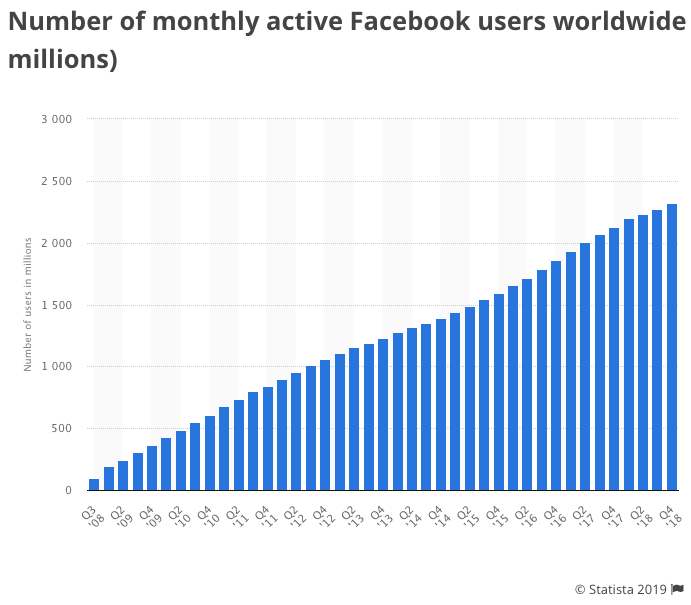
\includegraphics[width=\linewidth]{img/facebook-growth.png}
  \caption{Facebook Growth}
  \label{fig:FacebookG}
\end{figure}

In early 2000 is the year social media sites we know today started out and came into their own. Sites such as Facebook(2004), Reddit(2005) and Twitter(2006) all launched in the early 00's and are still very active today. These sites quickly gained an audience from people who wanted a more involved experience. These sites offered profile pages the user could customize and have users interact with one another. Facebook for example is the most popular social media site today (2019) expanding year over year in terms of users. 

Facebook has remained relevant through expanding their market and language options to make it more inclusive for people outside the western hemisphere where it first took off. which allowed it to incrementally increase its user-base year over year.

Sites early on like MySpace(2003), Flickr(2004) and Bebo(2005) all gained traction but rapidly fell out of use once more competition came into the market such as Facebook and Twitter.

\section{Modern Social Media}
Modern social media is constantly changing and is a market of "innovate or die". Social media sites are always trying to innovate in order to keep the audiences they've built over the years. An example is when Snapchat came into the market Facebook tries to create its own version of Snapchat stories in order to keep users on their platform.

Modern social media sites have their own perks that keep people using a different variety of social media sites and applications. Facebook is more of a personal social media between people you know or have met. Twitter is used to keep in up with people you would like to know about such as celebrities. Reddit is a post aggregator that is more of a classic forum from the early days of the internet. Instagram is a picture sharing application where you can follow friends and celebrities alike. All these social media site are different enough and offer a unique approach that they have been able to survive together. 

\section{Staying Relevant in our Ever-changing World} 


\begin{itemize}
\item Provide a context for your project.
\item Set out the objectives of the project
\item Briefly list each chapter / section and provide a 1-2 line description of what each section contains.
\item List the resource URL (GitHub address) for the project and provide a brief list of the main elements at the URL.
\end{itemize}
